% !TEX encoding = UTF-8 Unicode
% !TEX root = tese.tex

\chapter{Percurso}
\label{ch:percurso}


    \section{A música me levou à rede}
    
    Meus primeiros contatos com a World Wide Web foram em 1996, na época, tínhamos que ir até uma das salas em um laboratório da Poli, usar a rede em uns computadores Sun, já que não havia ainda servidores acessíveis em casa. Lembro, que minha atividade preferida na época era a coleta de letras de música, que eu imprimia e levava para a escola para cantarmos nos intervalos. Para ouvir música, no entanto, haviam as rádios, a MTV, uns poucos discos e CDs comprados ao longo dos anos e as fitinhas gravadas do rádio. O repertório acessível era muito reduzido, embora uma inclinação familiar para música ``séria'' garantiu um certo contato com um repertório tradicional da música contemporânea, jazz e música popular brasileira. Em casa, usava os computadores principalmente para jogar.


\todo[inline]{desenvolver sobre pirataria}
    \begin{citacao}
Comparados aos seus antecessores, as ambições dessa subcultura jovem aparentemente apolítica pareciam muito mais modestas: compartilhar músicas bacanas pela Internet. Entretanto, para a indústria da música, essa utopia hacker era um negócio desastroso. Pregar a revolução, tomar drogas e a perversão sexual eram práticas que podiam ser toleradas dentro desse empreendimento capitalista descolado. Tudo era permitido no maravilhoso mundo pop, com somente uma exceção: a música livre.\cite[370]{Barbrook2009}
\end{citacao}

Quando surgiu o Audiogalaxy (Figura \ref{fig:audiogalaxy}), que inaugurou a era dos softwares peer-to-peer, é que para mim ter internet realmente começou a fazer sentido. Na tela azul do site, um mapa de possibilidades que iam surgindo a cada download; o site oferecia um sistema de de sugestões, que mostrava outros artistas que ouvintes de uma determinada canção gostavam. Nesse período, consegui ter uma ampliação gigante do repertório, passando de uma centena de cds para milhares, descobrindo coisas tão diversas como as primeiras gravações de blues americanas, as várias nuances de música eletrônica do começo dos anos 2000 e a música popular brasileira. 

\begin{figure}
\centering
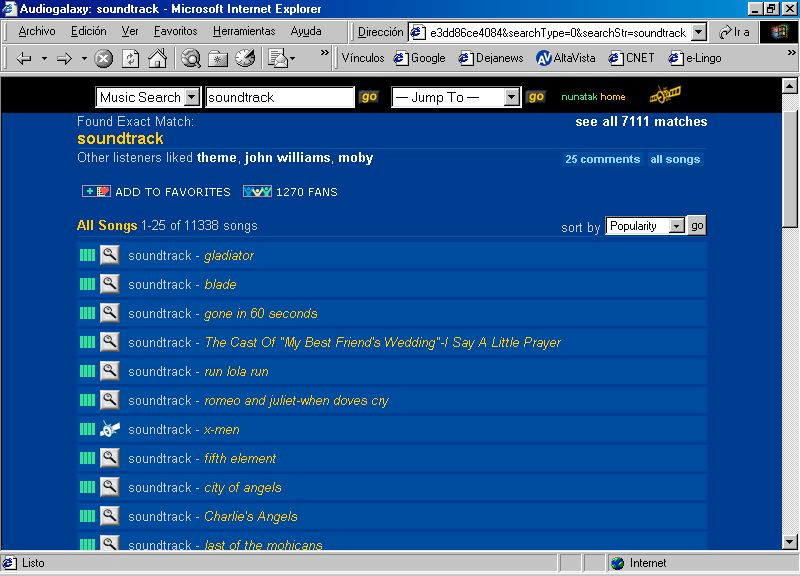
\includegraphics[width=1\textwidth]{pictures/cap1/audiogalaxy}
\caption{Interface do programa Audiogalaxy de compartilhamento de músicas.}
\label{fig:audiogalaxy}
\end{figure}


Com essa pesquisa de repertório adquirido na internet, através da nova cultura de dádiva que se estabelecia, acabei assumindo a posição de DJ em alguns happy hours quando em 2001 participei pela primeira vez da gestão do Gfau, o grêmio de estudantes da FAU, junto à chapa ``Estúdio 5''. Foi nesse ano também que comecei a desenvolver um interesse especial pelo design de interfaces, fazendo algumas experiências com animações em flash, entre elas o site para a Expofau 2001, que aconteceu naquele ano com cerca de 150 trabalhos inscritos. Mas ainda era para a mídia impressa que eu dedicava mais atenção e força de trabalho. Fiz uma iniciação científica bem técnica em design gráfico, investigando legibilidade de texto e me engajei em diversas comissões do Gfau, grupos de extensão e organizações estudantis dos quais fiz parte – Revista Caramelo, Jornal 1:100, Labhab Gfau, Grupo Anita Garibaldi, Revista Contravento e da fundação da Negação da Negação – pude experimentar com várias técnicas de composição gráfica digitais e analógicas. Foi uma época de extensa produção estudantil, do surgimento da ``Fau Paralela'', ``expressão dessa consciência de que a escola e o aprendizado estão em grande parte fora da instituição, do curricular'', como aponta Ana Carolina Ribeiro (2006) no seu TTG "trans Forma Ação, que analisa a produção gráfica da FAU na época \cite{Ribeiro2006}. 

Nessa época, comecei a desenvolver as primeiras pesquisas em composição gráfica modular, que chamava de ``Concretismo Tosco'', pela inspiração concreta e a precariedade no acabamento, uma influência do pensamento do arquiteto Sérgio Ferro, que defendia a manutenção do erro como um marca do trabalho na obra de arte \cite{FerroSergio2002}. 



Em 2005, o professor belga Etienne Delacroix veio ao Brasil oferecer a disciplina ``Oficina de Arte e Programação'' na Poli, que tive oportunidade de cursar como optativa. Ele instalou numa sala o Atelier Labs, uma mistura de laboratório e atelier, onde os alunos poderiam desenvolver projetos de seu interesse, relacionados com os temas que o professor nos apresentou, que iam de reciclagem de computadores, instrumentos musicais DIY, robôs, software livre e programação para web. O Atelier Labs foi um verdadeiro centro difusor de cultura livre em São Paulo, tendo colaborado com a formação de uma rede de ativistas em cultura digital que atuam até hoje em diversas cidades do Brasil. A proposta pedagócica do professor era de fazer com que os alunos conseguissem se embrenhar na caixa preta, desdevendando o funcionamento dos computadores e das lógicas de programação \cite{Delacroix2009}, para isso, fazia uso de computadores velhos que eram desmontados e re-configurados em torres, com seus compontentes à mostra. O Atelier Labs (Figuras \ref{fig:eti} e \ref{fig:eti2}) também se convertia em uma estrutura móvel que podia ser montado em lugares diferentes, acompanhando o professor onde ele precisasse.

\begin{figure}
\centering
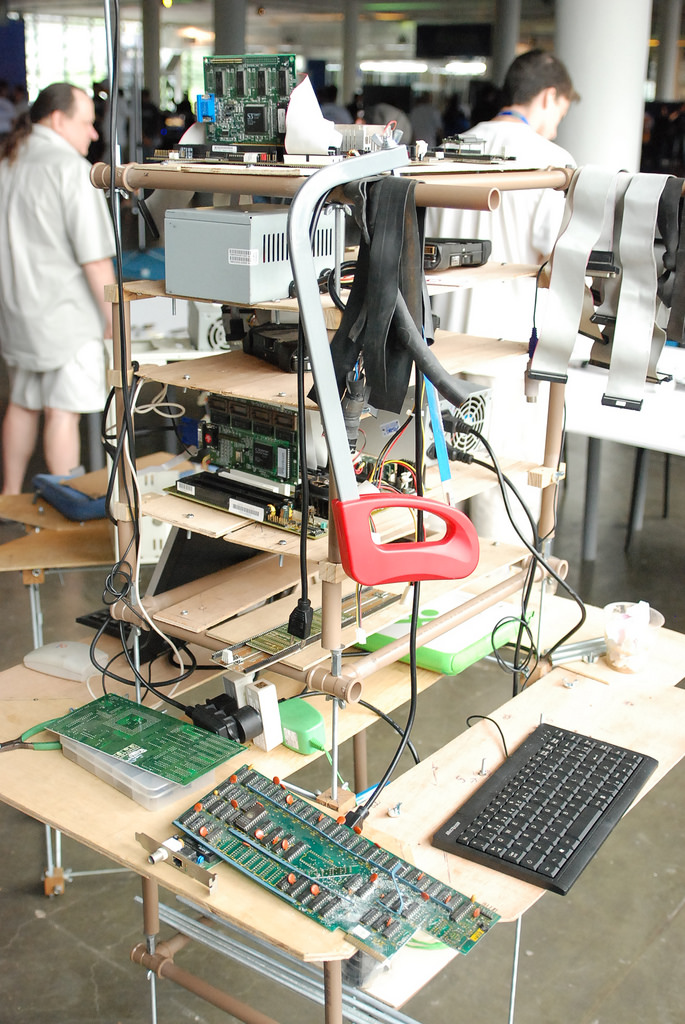
\includegraphics[width=1\textwidth]{pictures/cap1/eti1}
\caption{Ateliê móvel de Ethienne Delacroix.}
\legend{Fonte: Campus Party Brasil, 2008.}
\label{fig:eti}
\end{figure}

\begin{figure}
\centering
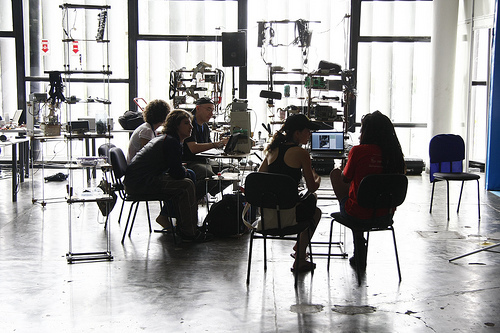
\includegraphics[width=1\textwidth]{pictures/cap1/eti2}
\caption{Aula da disciplina Ofina de Arte e programação, na Escola Politécnia.}
\legend{Foto: Fernando Cavalcanti.}
\label{fig:eti2}
\end{figure}


\section{A rede me levou à música}
O envolvimento nas atividades políticas estudantis, levou à participação em uma série de atividades musicais, inicialmente com a organização de festas, depois como percussionista no grupo Urbando, um núcleo do Gfau que atuava em festas e manifestações estudantis e posteriormente em atividades de livre improvisação que aconteciam às quintas feiras no gramado da FAU, o Som de Quinta. Esse engajamento me levou a uma paixão pela música como atividade prática e cotidiana, não mais somente como ouvinte. 

Comecei também a produzir música eletrônica, em um software que se chamava Jeskola Buzz, um software gratuito meio obscuro, que era usado por alguns artistas da cena eletrônica, funcionava uma plataforma aberta – embora não open-source – para a criação de instrumentos, chamadas machines, e oferecia uma ampla gama de sintetizadores e efeitos de áudio. O Buzz tinha uma interface bastante peculiar, que alternava três espaços:

\begin{itemize}
\item Um para estabelecer rotas de comunicação entre de processamentos de sinais digitais (DSP) (Figura \ref{fig:buzz1});
\item Um para desenhar padrões para os instrumentos e efeitos, que lembrava um cartão perfurado. Os parâmetros eram definidos em linguagem Hexadecimal e as notas no sistema de notação americano (Ex: C-3, etc) (Figura \ref{fig:buzz});
\item Uma linha do tempo, onde se podia distribuir os padrões desenhado ao longo do tempo (Figura \ref{fig:buzz3});
\end{itemize}

\begin{figure}
\centering
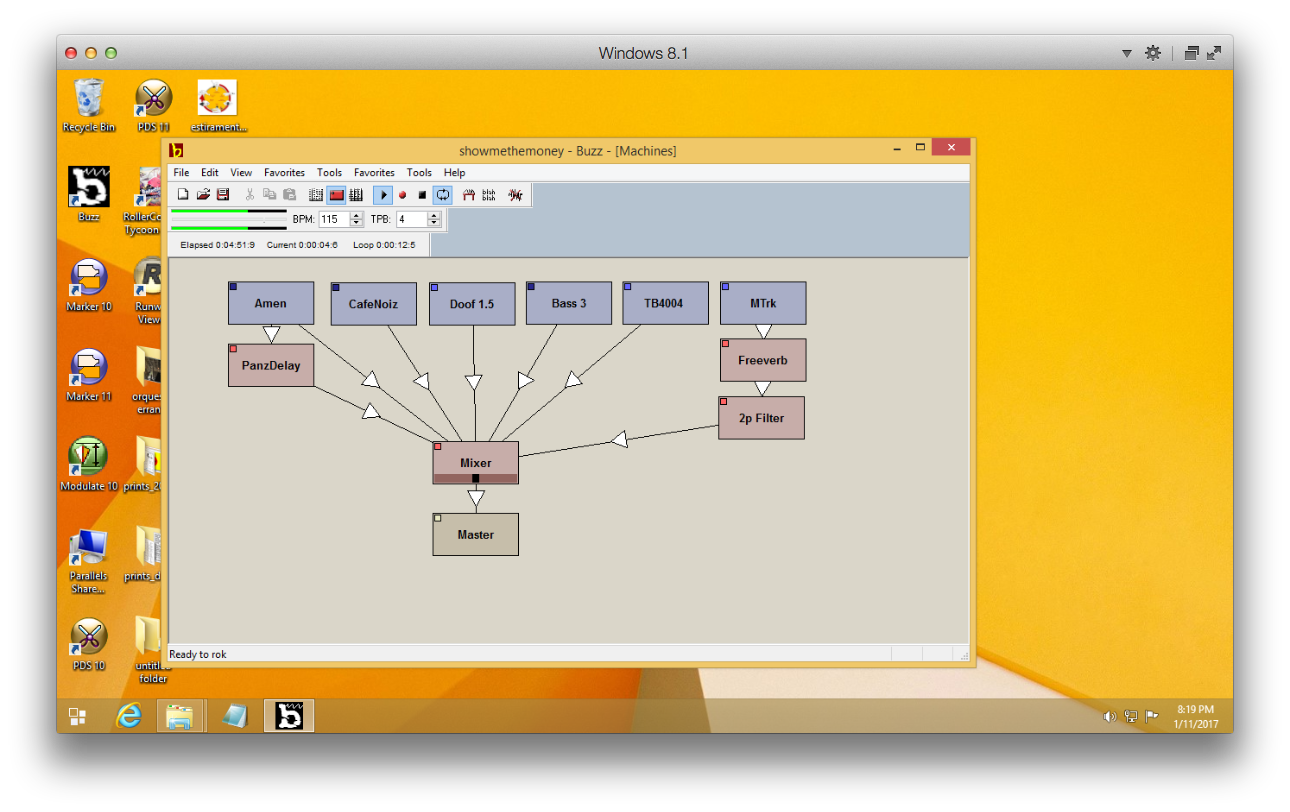
\includegraphics[width=1\textwidth]{pictures/cap1/buzz1}
\caption{Interface do programa Buzz.}
\label{fig:buzz1}
\end{figure}

\begin{figure}
\centering
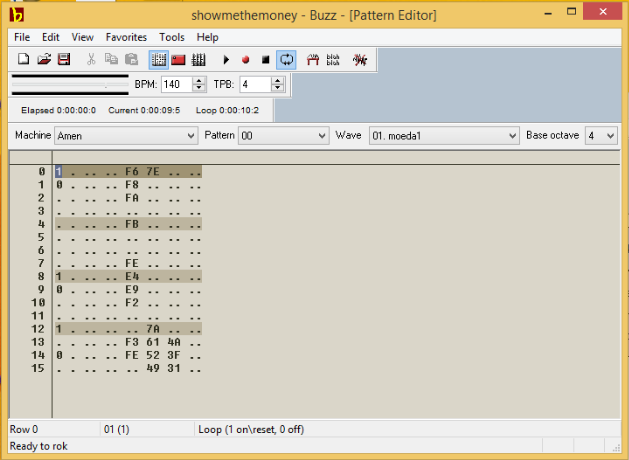
\includegraphics[width=1\textwidth]{pictures/cap1/buzz}
\caption{Interface do programa Buzz.}
\label{fig:buzz}
\end{figure}

\begin{figure}
\centering
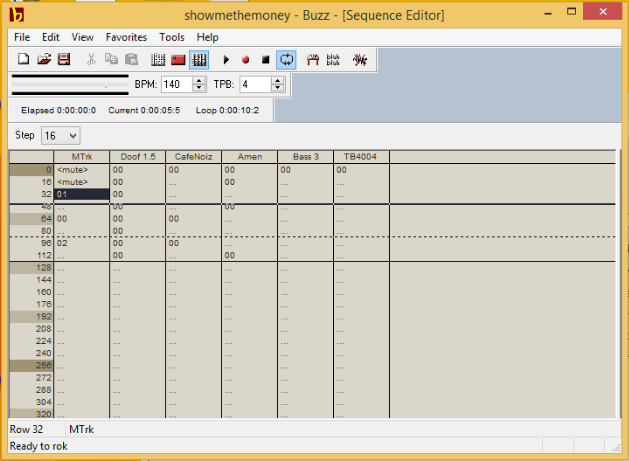
\includegraphics[width=1\textwidth]{pictures/cap1/buzz3}
\caption{Interface do programa Buzz.}
\legend{Fonte: screenshot da autora}
\label{fig:buzz3}
\end{figure}

Com ele, desenvolvi uma série de conhecimentos práticos em métodos de síntese e processamento de áudio, que organizei em experimentos sonoros metalinguísticos, chamados de Protomúsica. Metalinguísticos porque o próprio processo de composição levava em conta uma experimentação com os instrumentos e os materiais musicais, por exemplo:
Em estudo de harmonia e dissonância num ré. Disponível em: \url{http://finetanks.com/records/2005_2010/protomusica/estudo\%20de\%20harmonia\%20e\%20dissonancia\%20num\%20re.mp3} >, procurei explorar as possibilidades de intervalos musicais em um sintetizador aditivo;
Em Dodecafunk, procurei fazer uma batida funk com uma melodia que seguisse regras dodecafônicas. Disponível em: \url{http://finetanks.com/records/2005_2010/protomusica/dodecafunk.mp3}
Em percussiva, explorei as possibilidades de variação de timbre a partir de um padrão rítmico de apenas uma nota no sintetizador percussive FM. Disponível em: \url{http://finetanks.com/records/2005_2010/protomusica/percussiva.mp3}

Com o provedor, comecei a organizar um site para colocar materiais de produções minhas, e convidei alguns colegas que produziam também para publicar online no site Finetanks.com, que tinha também algumas ilustrações de Guilherme Garbato, minha pesquisa de iniciação científica, "Legibilidade e Evolução das Mídias, desenvolvida entre 2000 e 2001, e alguns primeiros experimentos em arte interativa; uns painéis modulares randômicos programados em php, inspirados nas obras de Athos Bulcão.  
Os primeiros projetos hospedados no Finetanks foram duas bandas punks, Os Otávios e Desprezíveis, de amigos do movimento estudantil, o Cabeça de Câncer, projeto de improvisação com Guilherme Garbato e Fernando Bizarri e o meu projeto solo de música eletrônica, Protomúsica. Com o tempo, foram anexados outros projetos como o JazzMetak e Freetools, de free jazz e Organograma, projeto de música eletrônica de Fernando Bizarri.

\begin{figure}
\centering
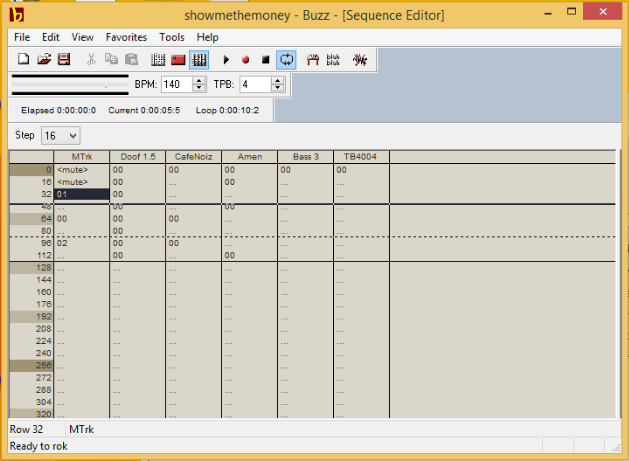
\includegraphics[width=1\textwidth]{pictures/cap1/buzz3}
\caption{Interface do programa Buzz.}
\legend{Fonte: screenshot da autora}
\label{fig:buzz3}
\end{figure}


\subsection{Cultura Digital}

Depois logo após a graduação, comecei a trabalhar como pesquisadora na equipe do Hacklab, um grupo de desenvolvedores web que atuava em São paulo financiados pelo projeto Cultura Digital, do Ministério da Cultura (MinC), para fornecer recursos para os pontos de cultura, que chegavam a 1000 unidades em 2006 \cite[6]{Lima2009}. Os pontos de cultura foram criados em 2004 na gestão de Gilberto Gil do MinC, para fomentar espaços culturais independentes em todas as regiões do país, ou segundo ele próprio Gil:
\begin{citacao}

``Para fazer uma espécie de do-in antropológico, massageando pontos vitais, mas momentaneamente desprezados ou adormecidos, do corpo cultural do País. Enfim, para avivar o velho e atiçar o novo. (Gil, 2003)" 
\end{citacao}


Entre os projetos que estavam sendo desenvolvidos pela equipe do hacklab estava o \url{Estudiolivre.org}, que tinha como objetivo ``a formação de espaços reais e virtuais que estimulem e permitam a produção, a distribuição e o desenvolvimento de meios de comunicação e de informação livres'' (idem, p. 12) e oferecia ferramentas para download e compartilhamento de arquivos de imagem, som e vídeo, além de manuals, fóruns e páginas pessoais, e é considerado um projeto pioneiro na cultura digital no Brasil. 

O trabalho no Hacklab me colocou em contato com grupos diferentes de pessoas atuantes nos circuitos de produção de cultura livre, em diferentes redes, como a Metareciclagem, Estudiolivre, Coletivo Coro, CMI e a Rede Saravá. Foi também uma época de intensa produção musical amadora, de marchinhas carnavalescas e músicas pop, muitas das quais não chegaram nunca a ser produzidas. 

\todo[inline]{cultura livre/pontos de cultura e cultura digital}

\subsection{Records}
Em 2010, comprei um gravador estéreo portátil e comecei a fazer algumas gravações em campo. Durante os festivais Submidialogias, em Arraial D'Ajuda e em Paranaguá e o Ruidocracia no Rio de Janeiro, gravei uma série de encontros musicais, jams e processos um tanto catárticos de improvisação e composição coletiva, em conjunto com Felipe Ribeiro, Jerônimo Barbosa, Fabiane Borges, Ricardo Brasileiro, Glerm Soares, Kaloan Menochite, entre outros. Passei então a editar o material gravado e transformei o Finetanks em uma pequena gravadora independente. Não havia suporte para áudio ainda na linguagem HTML, e para construir as páginas dos projetos era preciso inserir iframes com o endereço dos arquivos originais, processo que era relativamente trabalhoso e bastante artesanal, então, em 2010 o site foi transformado em um repositório, sem páginas em HTML para cada projeto, e o material passou a ser organizado em em subpastas, com os links diretos para os arquivos em mp3, sem nenhuma informação extra além do nome do arquivo, data de modificação e tamanho. 


\begin{figure}
\centering
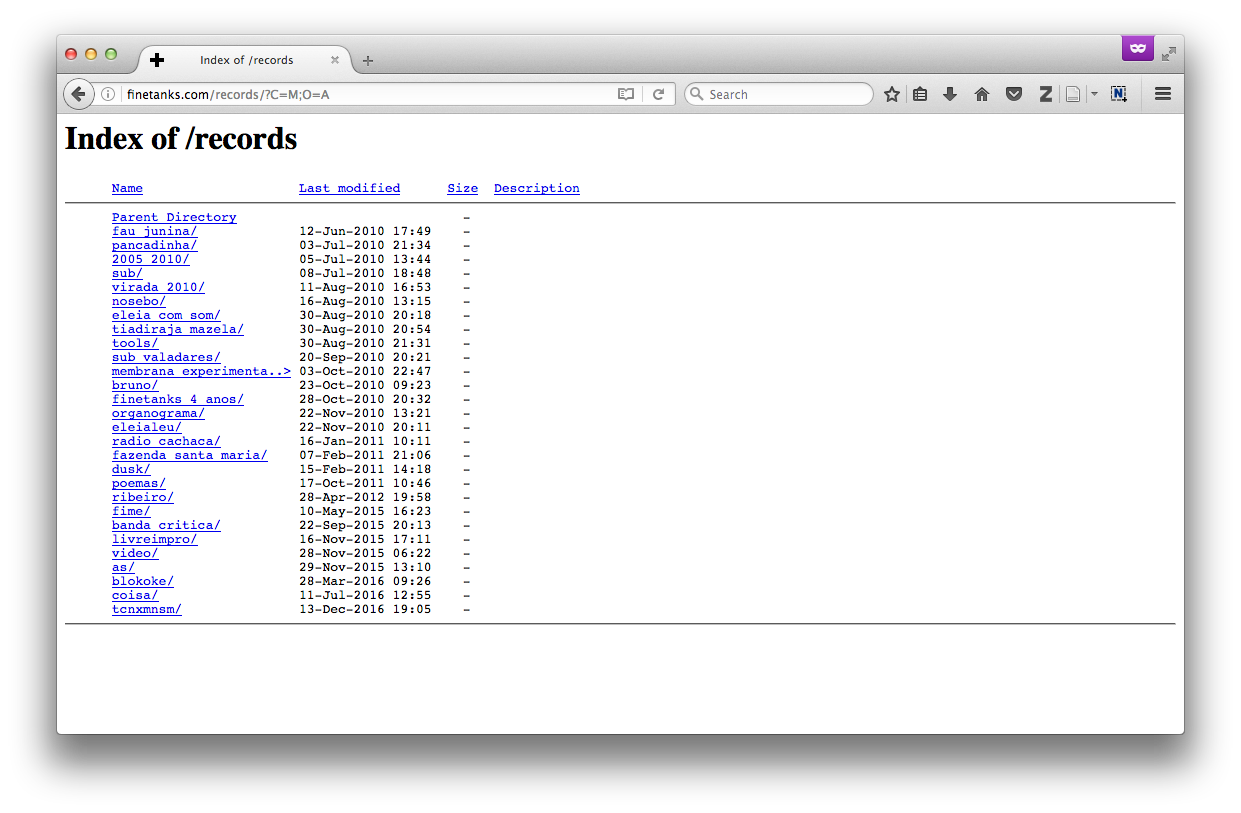
\includegraphics[width=1\textwidth]{pictures/cap1/finetanksrecords}
\caption{O endereço \url{http://finetanks/records} é o portal da gravadora, que não contém nenhuma página HTML, somente links para os arquivos em mp3.}
\label{fig:finetanksrecords}
\legend{Screenshot da autora, 6 de janeiro de 2017.}
\end{figure}


\begin{figure}
\centering
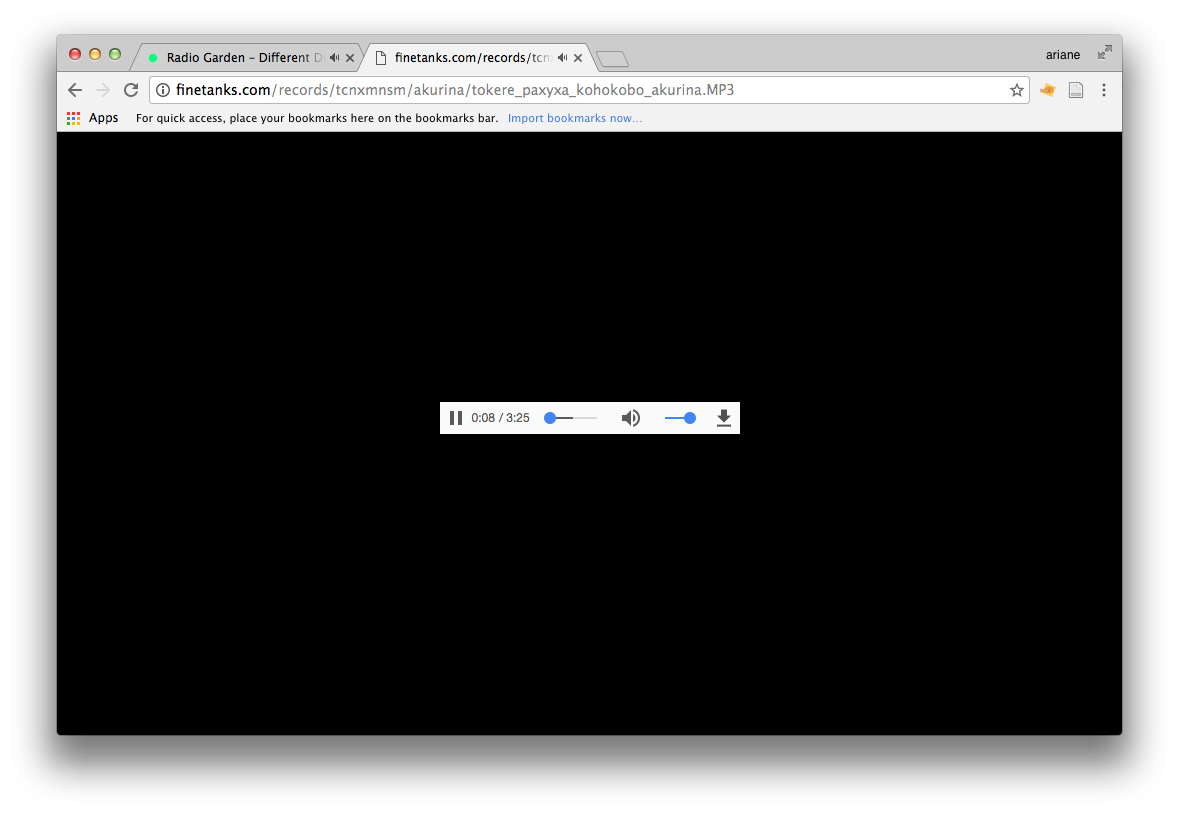
\includegraphics[width=1\textwidth]{pictures/cap1/finetanksmp3}
\caption{s arquivos de áudio são acessados pela interface padrão do navegador.}
\label{fig:finetanksmp3}
\legend{Screenshot da autora, 6 de janeiro de 2017.}
\end{figure}

Apesar de uma aparência até meio tosca, a estrutura é bastante funcional, pois permite um rápido compartilhamento e acesso, com muito pouco uso de dados, além de ser compatível com a imensa maioria dos sistemas e dispositivos, é, como a estrutura exposta de um edifício brutalista. Surpreendentemente, quando removemos as páginas HTML, a audiência do site aumentou bastante, chegando a 2000 acessos diários em 2011 e até hoje ainda contando com uma média de 600 acesso por dia.

Entre 2010 e 2011 editei e postei músicas do festival de Submidialogias de Arraial D'Ajuda e do Ruidocracia no Rio de janeiro (\/sub\/); das apresentações com o Coletivo 24h do projeto Cromocinética, que desenvolvi em puredata e Buzz Machines em conjunto com Fernando Bizzarri (Organograma) e Amer Moussa, e de Ricardo Carioba, na Virada Cultural no MIS (virada\_2010\/); apresentações musicais no sebo Elea com Gabriel Kerhart, Rômulo Alexis e Felipe Ribeiro (nosebo\/); arquivos da banda (tiadiraja\_mazela\/) de Kaloan Menochite e Pilantropov Pausanias, gravações do ritual final de encerramento do festival de Submidialogias de Paranaguá, com participação de Glerm Soares, Felipe Ribeiro, Fabiane Borges, Roger Bagé, Lucida Sans e membros da comunidade caiçara da ilha (\/sub\_valadares\/); jam sessions do grupo Membrana Experimental Fiat Lux, coordenados por Rômulo Alexis e Leila Monsegur (membrana\_experimental\_fiatlux\/); gravações de Bruno Araújo (Walter Rego), em seções de improvisações de rap no Gfau (bruno\/) e seção no piano com Marco Aurélio Lagonegro; a apresentação de Retrigger na festa de aniversário de 4 anos do site (finetanks\_4\_anos\/); diversas gravações dos encontros Eleia leu, organizado por Gabriel Kerhart, na biblioteca Alceu Amoroso Lima e na galeria Bordô, que inclui participações de Amélia Monteiro, Ana Gold, Bruno Schiavo, Gabriel Kolyniak, Diego Sampaio, Marcelo Maccaferri, Felipe Ribeiro entre outros (\/eleialeu\/) até as gravações feitas na Fazenda Santa Maria, de Thereza Amaral, que incluiu uma experiência lisérgica pesada que que envolveu um certo grau de incorporação, que batizamos de Exu na Cozinha (\/fazenda\_santa\_maria\/), uma experiência que foi bastante catártica e de certa forma amedrontadora. 
Interrompi as atividades do selo por um tempo após ter o gravador digital furtado depois de uma apresentação solo realizada no 2o Festival \#Dis Experimental, tendo retomado somente em 2015, depois de iniciar as pesquisas neste doutorado. A essa altura, também já havia uma série de ferramentas para publicaçnao onlinde de conteúdo, como SoundCloud e Youtube, onde os próprios artistas podem alimentar com conteúdo, e a gravadora já não era mais tão necessária.

Apesar todo esse interesse em música e de começar a estabelecer uma produção voltada para ela, o campo disciplinar onde estava inserida como pesquisadora ainda era o do design, e a partir dele comecei a desenvolver algumas práticas em vídeo e música visual. Em parceria com Amer Moussa, no Coletivo 24h, fizemos em 2009 experimentos com colagens de vídeos como Pink Flamingos, Copacabana Mon Amour e A Mulher de Todos, sobrepostas a animações geométricas psicodélicas, que apresentamos na festa Perversa, no clube Glória (Perversa hum 01 - Coletivo 24h). Na época, fazíamos as animações em flash, e utilizamos softwares de edição de vídeo para criar vídeos estáticos, inspirados em trabalhos como os de Marcel Duchamp e Norman McLaren. 

\subsection{Pure Data}

Pure Data
A experiência prática junto ao Hacklab em software livre me fez propor ao recém inaugurado Lab-C, no Centro Cultural da Juventude da Prefeitura Municipal de São Paulo (PMSP), que procurando desenvolver a ``produção cultural integrada às práticas de difusão do conhecimento a partir do uso de softwares livres'', oferecia oficinas práticas de ``metareciclagem, áudio, vídeo, rádio e gráfico" \cite{PMSP2008}, duas oficinas de design gráfico baseadas em software livre. Desenvolvi uma oficina que sintetizava os conteúdos das duas, onde sempre procurava apresentar um certo repertório da história do design como El Lissitzky, Alexandr Rodchenko, Josef Muller Brockmann, Paul Rand, Aluízio Magalhães, Rogério Duarte e César Vilela, alguns conceitos teóricos de Gestalt e Semiótica, e questões técnicas como tipografia e diagramação, realizando exercícios práticos como fazer uma capa de disco, um flyer, um cartaz, de acordo com os interesses dos grupos majoritariamente de jovens que frequentavam a oficina. 

Nesse período, pude participar também participar da oficina ``DESIGN E INTERAÇÃO SONORA'', Ministrado por Giuliano Obici:
\begin{citacao}
Curso de programação e invenção musical com o intuito de apresentar conhecimentos técnicos e teóricos sobre o áudio no meio digital e de alguns dispositivos como microfone, interfaces, controlador MIDI, sensores e circuitos envolvendo o ambiente de programação Pure Data (PD). \cite{PMSP2008}
\end{citacao}

O ambiente de programação Pure Data (Pd), assim como o Max, oferece a possibilidade de programar processos de síntese e controle de áudio vídeo e dados, em uma interface gráfica que interliga objetos representados por caixas de texto através de linhas em uma tela, possibilitando ao programador controlar fluxos de informação em um esquema de hierarquias semelhante aos diagramas de arquitetura de informação. Essa possibilidade de programação visual foi bastante estimulante, pois a linguagem de blocos interligados que sua interface oferecia era um tanto semelhante à do Buzz, e para mim era mais fácil de compreender do que a programação por escrito, pela visualidade da informação. Ao mesmo tempo, a lógica era totalmente diferente; enquanto o Buzz é uma ferramenta de composição linear, com linha do tempo e instrumentos pré-programado, Pd é um ambiente de programação complexo, cuja interface, como analisamos no artigo ``Graphic Interfaces for Computer Music: Two Models'', não comunica muito ao usuário o que se é possível fazer \cite{Stolfi2016}. 
Em 2009 aconteceu uma conferência internacional de Pd em São Paulo, onde pude entrar em contato com uma série de trabalhos inovadores em arte sonora e música experimental, como os trabalhos dos duos CHDH de Cyrile Henry e Nicolas Montgermont (Figura \ref{fig:chdh}), que tocam um sintetizador audiovisual com correspondência entre os processos de síntese sonora e de movimento e Hp-Process de Philippe Boisnard e Hortense Gauthier (Figura \ref{fig:hp}), onde a performer nua e grávida era transposta para dentro de um universo poético tipográfico construído em 3 dimensões e manipulado em tempo real através de sensores adaptados de kinetics e interface em Pure Data. 

\begin{figure}
\centering
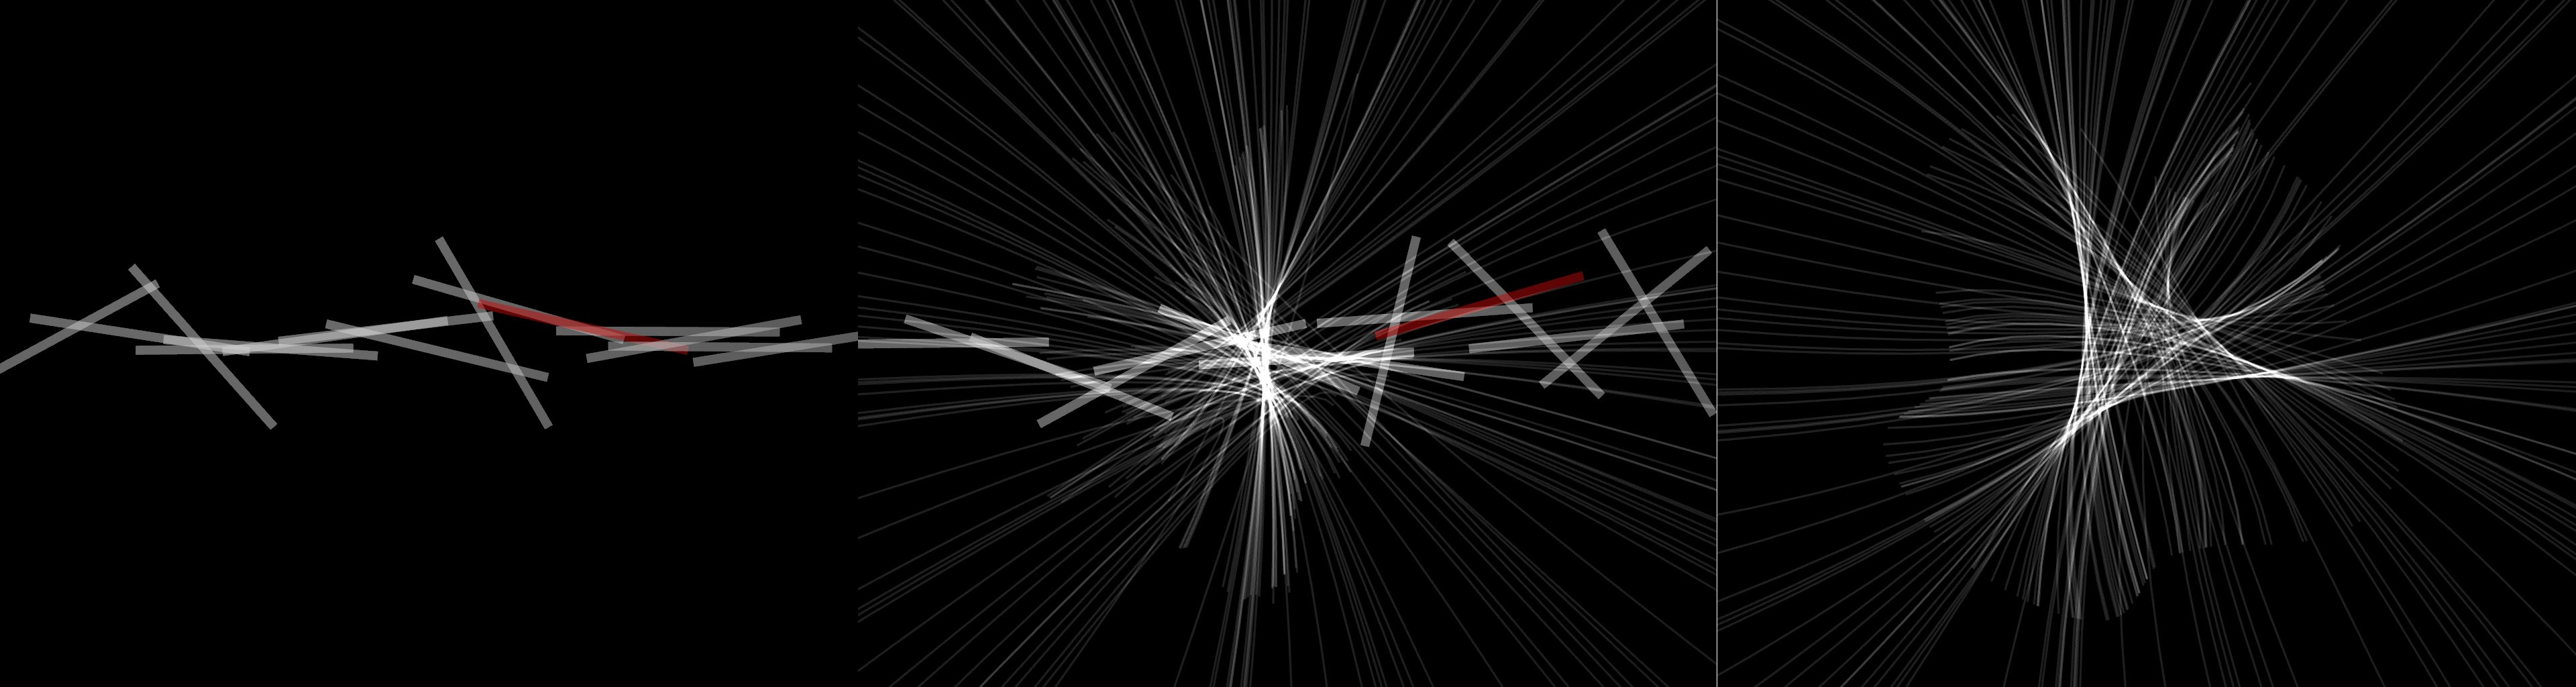
\includegraphics[width=1\textwidth]{pictures/cap1/CHDH}
\caption{Detalhes da performance Eggregore, do grupo CHDH apresentada na PdCon em 2009.}
\label{fig:chdh}
\legend{Fonte: \url{http://chdh.net/egregore.php}}
\end{figure}

\begin{figure}
\centering
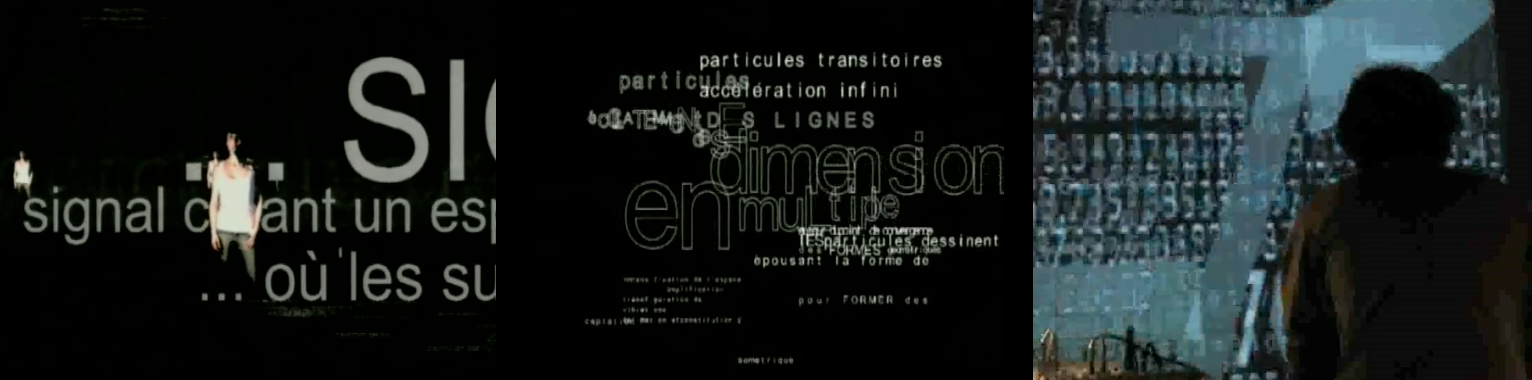
\includegraphics[width=1\textwidth]{pictures/cap1/hp1}
\caption{Detalhes da performance HP Process, apresentada na PdCon de 2009.}
\label{fig:hp}
\legend{Fonte: \url{http://databaz.org/xtrm-art/?p=439}}
\end{figure}

A partir desse contato, comecei a desenvolver um patch para processamento de áudio e vídeo em tempo real, que foi utilizado nas performances do projeto Cromocinética do Coletivo 24h. O patch interligava até três computadores: em um deles era feito o controle da ordem dos vídeos, a partir de uma biblioteca de loops de vídeo produzidos por Amer Moussa; no outro era controlado o som, produzido por Fernando Bizarri (Organograma) no Buzz; o Buzz enviava o sinal de áudio e informação MIDI para um terceiro, onde se controlava as formas geométricas que eram processadas em tempo real a partir do envelope sonoro do áudio, passando por um filtro que separava as frequências graves e as agudas, gerando sempre uma composição de formas diferentes – mas sempre muito concretas – em movimento frenético sincronizado com o áudio. Um trecho do vídeo da performance ocorrida no MIS está disponível no youtube em:  \url{https://www.youtube.com/watch?v=_ZsqAX7roBM}.

\begin{figure}
\centering
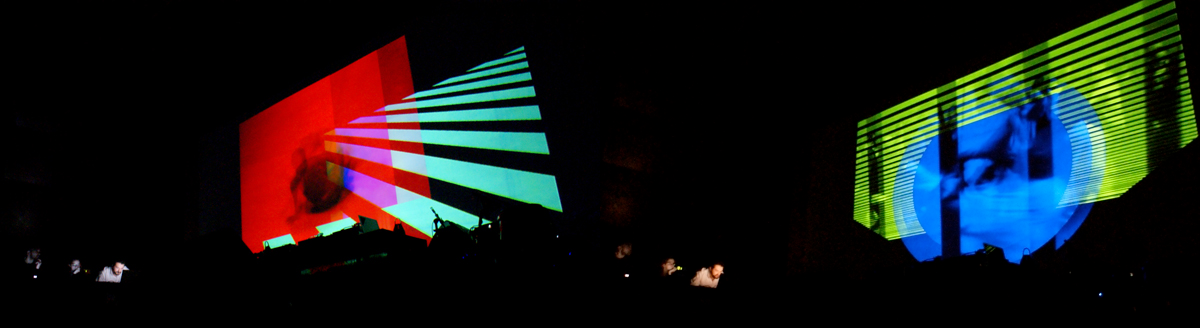
\includegraphics[width=1\textwidth]{pictures/cap1/cromocinetica}
\caption{Fotos da performance audiovisual Cromocinética.}
\label{fig:cromocinetica}
\legend{Fonte: \url{http://databaz.org/xtrm-art/?p=439}}
\end{figure}

O patch foi construído de forma modular. Comecei desenvolvendo figuras mais simples, como os círculos e triângulos até chegar em estruturas mais complexas como grids e listras, conforme ia desenvolvendo o aprendizado em programação no software. Essas primeiras experiências com Pd começaram a tornar a possibilidade pesquisa na música mais palpável, mas ainda estavam muito distantes do percurso acadêmico que estava percorrendo até então, que tinha como questão central a world wide web e suas tecnologias.

\subsection{Essa é pra tocar}
Quando fui convidada por Daniel Scandurra e Gabriel Kerhart para pensar no desenvolvimento de uma obra de arte interativa para compor a exposição Gil 70, de curadoria de André Vallias, em comemoração dos 70 anos do cantor Gilberto Gil, que aconteceu em 2014 O Daniel estava desenvolvendo um projeto chamado Moisacages\footnote{http://mosaicages.blogspot.com.br/}, onde compunha mosaicos com vários vídeos no Youtube, para serem tocados simultaneamente pelos visitantes de seu blog, e a idéia era produzir alguma obra interativa nesse sentido. Pensamos em construir uma espécie de instrumento audiovisual que funcionasse como uma máquina de montagem a partir de fragmentos sonoros.

Era importante para nós que a obra fosse interativa em um sentido imersivo, que convidasse o público a participar e desse possibilidade de se passar um tempo mergulhado, e não queríamos que fosse uma coisa que ficasse soando constantemente durante a exposição, uma obra viva que só funcionasse a partir de uma ação concreta. 

Naquele ano, haviam sido lançadas as especificações do HTML5 e o navegador Firefox tinha passado a dar suporte à tag <audio> em páginas da internet, o que abriu perspectiva para desenvolver a obra diretamente usando um navegador de internet como suporte. Pensamos em criar uma página que funcionasse como um instrumento musical, onde o público poderia compor com fragmentos da obra do cantor, criando novas sonoridades a partir da sobreposição de samples. 
Como designer, atuando na produção de jornais e revistas acadêmicas durante a graduação, um processo que foi fundamental na prática compositiva de grupos que participei foi o da fotomontagem, especialmente durante a produção da Revista Contravento HUM!. Usávamos uma técnica de fotomontagem com recortes de xerox, apresentada pelo professor Vicente Gil Filho, que, em oposição ao computador, que é uma ferramenta de uso individual, permitia que uma equipe de pessoas trabalhasse de forma coletiva com os mesmos materiais, manipulando-os na mesa, na sala do Gfau. Posteriormente, como docente na Universidade Nove Julho, ministrando a disciplina Projeto da Imagem, utilizava a mesma técnica em para exercícios onde os alunos deveriam desenvolver imagens que pudessem transmitir certos conceitos de linguagem visual. O que eu constatei foi que, se a base original de imagens apresentadas para as montagens fosse consistente, a qualidade estética dos trabalhos apresentados melhorava significativamente. 
Um princípio semelhante poderia ser utilizado para pensar em montagem sonora, procurando trechos significativos que funcionassem de maneira autônoma, fazendo uma seleção de um repertório prévio. Fizemos uma varredura na obra musical de Gilberto Gil, separando fragmentos de som que dividimos em 6 diferentes grupos: 

\begin{description}
\item[falas,]{ como trechos de discurso e falas significativas, sem som de fundo;
}
\item[gilbertália,]{ que reunía tudo que fosse relacionado à outras pessoas, como gil cantando outros compositores;
}
\item[banda,]{ com trechos de canções com fundo musical com banda;
}
\item[voz e violão;]{}
\item[onomatopeias,]{ com trechos de gritos, berros, ou outros sons curtos muito característicos do cantor;}
\item[bases,]{ com trechos de áudio mais longos; 
}

\end{description}


Pensamos em uma estrutura em seis faixas, em uma referência ao I CHING, que chamamos de ``Hexagrama Essa é pra tocar''.  Cada faixa correspondia a uma categoria de samples, de modo que na tela sempre haveria a possibilidade de combinar arquivos de grupos diferentes. Desenvolvi uma estrutura em JavaScript que separava cada faixa de samples em arquivos HTML diferentes, de forma que os arquivos pudessem ser desenvolvidos em paralelo e um sistema de códigos para estilos e tamanho de texto que possibilitou que toda equipe trabalhasse diretamente no código, mesmo sem ter conhecimentos desenvolvidos em HTML. 
Cada arquivo HTML correspondia a uma faixa do hexagrama, que por si continha muitos samples. As faixas podiam ser arrastadas continuamente para cima e para baixo, infinitamente, de modo a permitir variadas combinações entre as elas, mas oferecendo sempre um número limitado de possibilidades na tela. Para criar esse efeito de rolagem infinita era necessário multiplicar os elementos na tela, então para não sobrecarregar o sistema, os objetos de áudio ficavam todos em um arquivo separado, e apenas as faixas eram processadas em tempo real manipuladas. 
Desse modo, conseguimos chegar em cerca de 800 samples de áudio, que na tela eram representados por trechos das letras, imagens ou símbolos, e GIFs animados. quando tocados, alguns dos samples disparavam em conjunto vídeos, que convidamos o videoartista Gregório Grananian para fazer, que podiam ocupar toda a tela ou parte dela. Os GIFs às vezes se sobrepunham aos vídeos,  criando uma montagem audiovisual em tempo real, uma espécie de cinema expandido. 

\begin{figure}
\centering
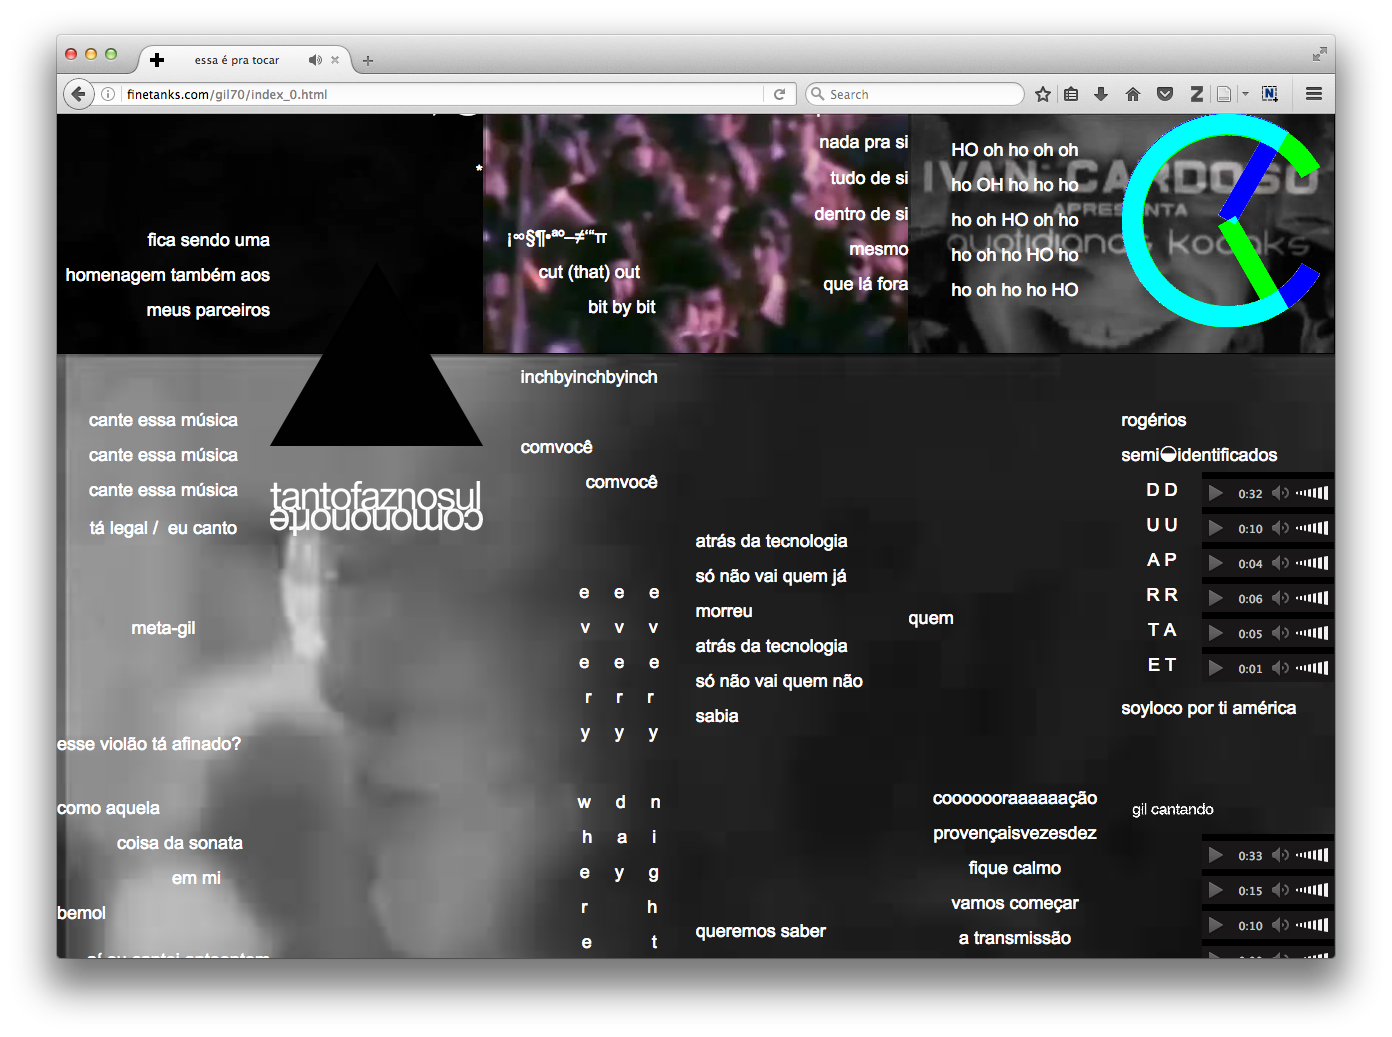
\includegraphics[width=1\textwidth]{pictures/cap1/gil701}
\caption{Interface do projeto ``Hexagrama essa é pra tocar''.}
\label{fig:gil701}
\legend{Fonte: Screenshot da autora}
\end{figure}

\begin{figure}
\centering
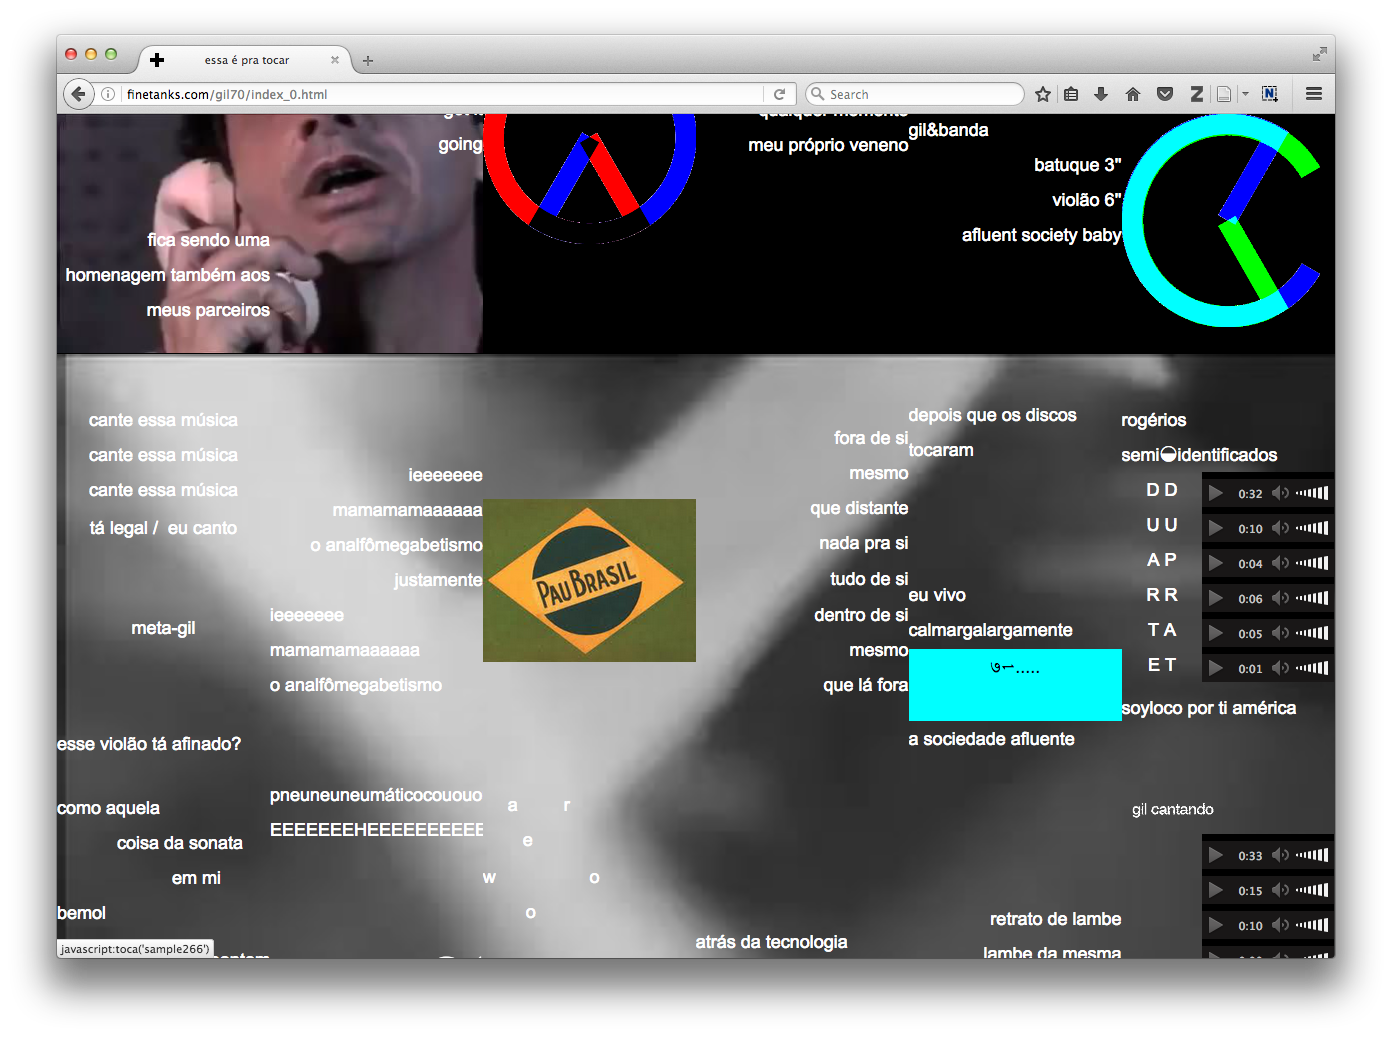
\includegraphics[width=1\textwidth]{pictures/cap1/gil702}
\caption{Interface do projeto ``Hexagrama essa é pra tocar''.}
\label{fig:gil702}
\legend{Fonte: Screenshot da autora}
\end{figure}

Durante a exposição, o site rodava em um totem com tela sensível ao toque no Firefox, a partir de arquivos em um computador local, sem necessidade de internet. Por ser baseado somente em HTML, CSS e JavaScript, o Hexagrama não depende de nenhuma tecnologia de processamento no servidor, então é bastante portável, podendo ser tocado diretamente de um pendrive, por exemplo. Isto facilitou sua montagem nos diversos locais onde foi exposto. Apesar de ter sido pensado como uma instalação interativa, existem algumas versões online que podem ser utilizadas abertamente até hoje. \footnote{Disponível em: \url{http://finetanks.com/gil70}.}
Além do totem com tela sensível ao toque, onde o público interagia com a obra, nas exposições no Rio de Janeiro, no Centro Cultural dos Correios e em São Paulo, no Itaú Cultural, usamos também um projetor, que reproduzia o site em tamanho grande e duas caixas de som omnidirecionais, que contaminavam todo ambiente expositivo com os sons disparados pela obra.

Esta primeira experiência em arte sonora baseada em tecnologias web, que também foi uma experiência de desenvolvimento de um projeto de interface de invenção, foi a ponta de lança para esse projeto de pesquisa. A partir da constatação práticas dos potenciais do uso de HTML, CSS e Javasçript, tendo o navegador como suporte, comecei a pensar na ideia de desenvolver instrumentos musicais, e isso pareceu o caminho que poderia unir o meu percurso de pesquisadora em design de interfaces web, que segui durante o mestrado, com o interesse nas práticas musicais, sobretudo experimentais, que estava desenvolvendo.


\newpage